\part{Build a job monitor}\label{part-workshops}
\chapter*{A route through the working example}
\addcontentsline{toc}{chapter}{Introduction: A route through the working example}

This part gives the collection a practical spine. Seven workshops follow one useful application from job identities and immutable state to four presentations, keyboard ownership, asynchronous results, constrained geometry, behavioral evidence and a reproducible source package. The application is small enough to inspect and large enough for the design principles to encounter real tradeoffs.

\section*{Build, break, test and ship}
\subsection*{One task, several pressures}

The job monitor carries status, progress, filtering, logs, failure and cancellation. Its work is simulated, so the example can concentrate on the architecture of a terminal application. The same facts must remain understandable in interactive, static/CI, pipe and accessible presentations. Several exercises deliberately violate those requirements before showing the production repair.

\subsection*{Use the checkpoint that belongs to the page}

The separate companion repository is pinned to published Bijou 7.2.0. Its checkpoints, tests, exact edition commit and limitations are recorded near the front of this book and in the companion. The historical source chapters retain their own versions and context. Read a workshop for a runnable teaching path; read the later records for the history and reasoning behind a particular contract.

\chapter{Workshop 1: A job worth monitoring}\label{workshop-01}

\section{Start with the user's question}

A person starts a build and wants to know whether it is making progress, whether it failed, and whether it is safe to leave. The job monitor in these workshops gives those questions a concrete home. It has three jobs: compile the application, run the tests, and publish the package. These are simulated jobs driven by scheduled events. The example never invokes a build tool or publishes anything. That boundary keeps the lesson about terminal application design while leaving room for a real process adapter later.

\subsection{Facts before decoration}

A job has a stable identity, a title, a textual status, a percentage and a run identity. Failure can also carry an explanation. The run identity distinguishes two attempts at the same job; a percentage alone cannot do that. Selection belongs to the monitor, rather than being inferred from where a highlight happened to be painted.

The \texttt{Job} class checks its invariants when a value is created. A successful job must be complete. Progress must be a finite number between zero and one hundred. A run identity is a non-negative integer. An immutable job can be handed to a renderer or retained in a test without a later update silently changing the value under examination.

\VerbatimInput[formatcom=\sourcecodefont,fontsize=\fontsize{12}{13}\selectfont,breaklines,breakanywhere]{companion-snippets/job.ts.txt}

\subsection{What immutability costs}

Each transition constructs a new job or monitor snapshot. That adds allocation and some copying. For three small jobs, the cost is easy to understand and measure. For a monitor with hundreds of thousands of entries, the collection strategy would need another decision. Immutability establishes an ownership boundary; it does not exempt a program from measuring its workload.

\section{Keep meaning out of the presentation}

A failed job remains failed when the terminal loses color. A running job remains running when a narrow viewport requires a different layout. The domain model therefore stores statuses such as \texttt{running} and \texttt{failed}, not color names, terminal escape sequences or coordinates.

\subsection{A tempting shortcut}

It is tempting to store preformatted rows as the application's state. That works until filtering needs the job identity, cancellation needs its run, or a pipe consumer needs a numeric percentage. Parsing those facts back out of painted text reverses the dependency. Here, presentation consumes the facts. Commands and tests use those same facts directly.

\subsection{Run the first checkpoint}

From the companion repository, run \texttt{npm ci}, then \texttt{npm run checkpoint -- 01}. The output contains three queued jobs. Read the rows with color disabled and answer: which job is selected, what state is each job in, and how much work is complete? The initial checkpoint introduces \path{src/job.ts}, the initial monitor snapshot, and the static presentation. The next workshop reuses that snapshot rather than inventing a separate model for each environment.

\section{Try a real extension}

Add a job whose title contains a wide character and a combining accent. Give it an identity that remains stable if its title changes. Success means the same identity reaches every presentation and every transition. A title is a label for people; changing its spelling must not redirect an asynchronous result to another job.
%
\chapter*{Workshop 2: One application, four environments}\label{workshop-02}
\addcontentsline{toc}{chapter}{W2: One application, four environments}

\section{Hold the task constant}

Run \texttt{npm run checkpoint -- 02}. Every presentation receives the same fixture: compilation succeeded, tests failed with an explanation, and publication is forty percent complete. Changing a presentation must not change those facts. The following specimens come from the companion's actual formatter and Bijou 7.2.0; they use Recursive Mono for the terminal cell projection. They are complete fixture outputs wrapped at forty cells for print. The interactive specimen shows presentation content; input routing and the runtime viewport are introduced in Workshop 3.

\subsection{Interactive and static}

\begin{minipage}[t]{.48\linewidth}
{\headingfont\large Interactive\par}\smallskip
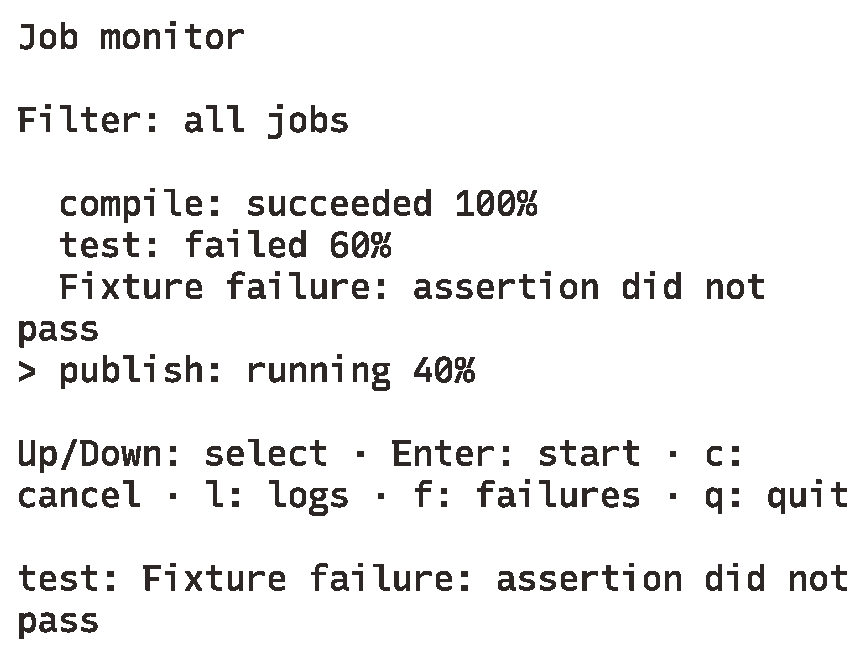
\includegraphics[width=\linewidth]{figures/monitor/monitor-interactive.pdf}
\end{minipage}\hfill
\begin{minipage}[t]{.48\linewidth}
{\headingfont\large Static / CI\par}\smallskip
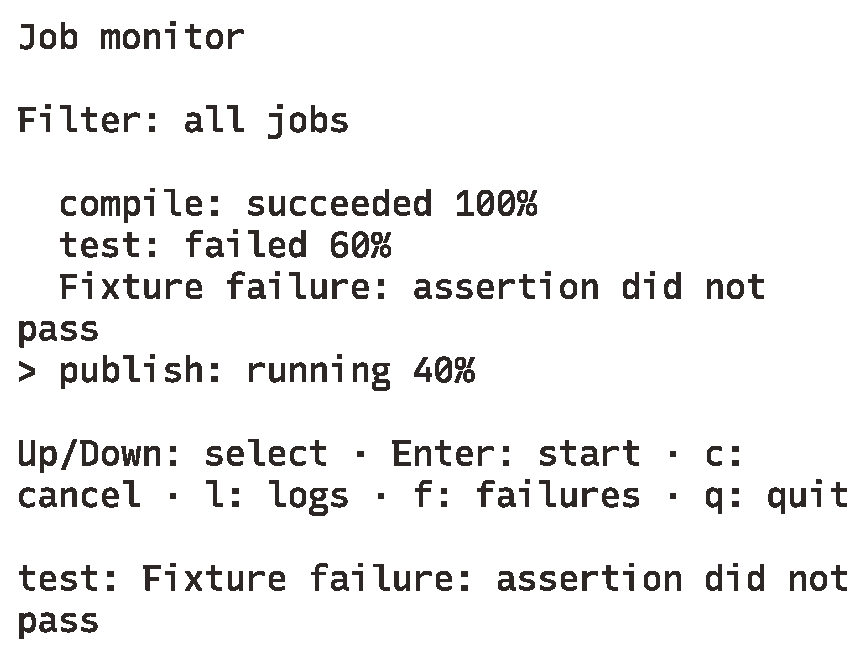
\includegraphics[width=\linewidth]{figures/monitor/monitor-static.pdf}
\end{minipage}

The rich mode provides an application loop in a terminal. Static mode emits a snapshot suitable for a CI log or a saved report. The two narrow specimens deliberately share a compact textual layout. The important difference is the delivery contract: a static invocation writes once and exits; an interactive invocation accepts input and redraws a viewport.

\subsection{Pipe and accessible}

\begin{minipage}[t]{.48\linewidth}
{\headingfont\large Pipe\par}\smallskip
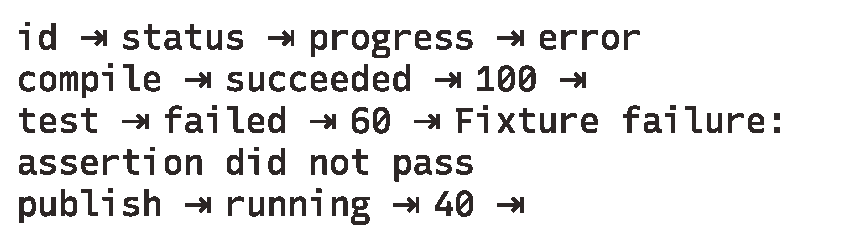
\includegraphics[width=\linewidth]{figures/monitor/monitor-pipe.pdf}
\end{minipage}\hfill
\begin{minipage}[t]{.48\linewidth}
{\headingfont\large Accessible\par}\smallskip
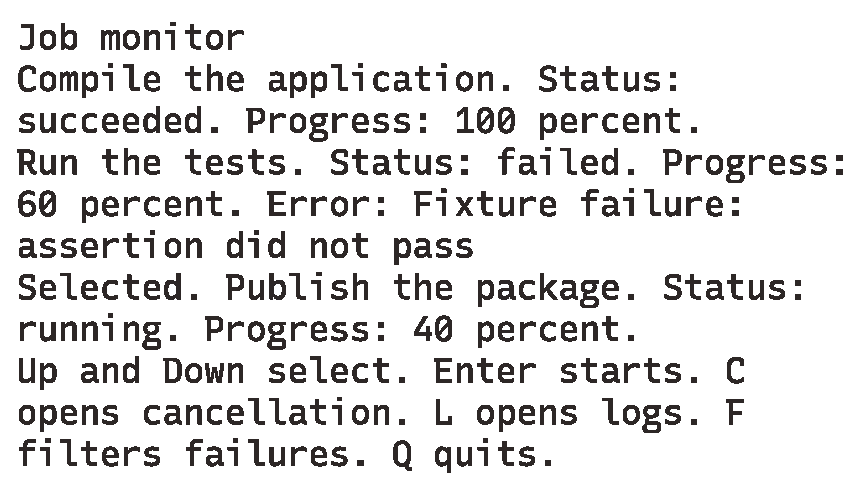
\includegraphics[width=\linewidth]{figures/monitor/monitor-accessible.pdf}
\end{minipage}

The pipe specimen makes tab characters visible as \texttt{⇥} for print. Its original TSV output is retained with the capture. It has stable identifiers, textual statuses, numeric progress and a separate error field. It has no cursor controls, decorative frame or keyboard help. The accessible presentation spells out selection, state, progress and the available actions. That is an explicit alternative presentation, not a claim that an automated text check establishes usability with every screen reader.

\section{Degrade honestly}

\subsection{Preserve the answer, choose the form}

A narrow terminal may replace a multi-column table with one compact record per job. A pipe should replace visual relationships with a stable serialization. An accessible view should state a selected relationship that a highlighted row might otherwise imply. In each case, ask what the reader still needs to understand and accomplish. The invariant is the task's useful meaning.

\subsection{Choose mode and styling separately}

The companion uses an explicit \texttt{--mode} choice when provided. Otherwise, redirected output chooses pipe mode; a CI environment attached to a TTY chooses static mode; an ordinary TTY chooses interactive mode. \texttt{NO\_COLOR} controls styling. It is not an instruction to erase interaction or replace a record format. These are application decisions made around the pinned Bijou API, not an assumption that every historical release detected modes in the same way.

For exact TSV without npm's script banner, use \texttt{node --import tsx src/main.ts --mode=pipe > jobs.tsv}, or npm's silent form documented in the companion. Inspect the saved file with a tab-aware tool. A terminal screenshot cannot establish that a data stream has the right number of fields.

\section{Break meaning before repairing style}

Run \texttt{npm run exercise -- color}. It fails because a colored dot is the only failure indication. Remove the color and the assertion has nothing useful to read. Diagnose the missing fact, then run with \texttt{--repair}. The repair uses a textual status. Color can reinforce that word later. Its cost is a less compact display; its benefit is that failure survives monochrome output, copying and speech.
%
\chapter{Workshop 3: Follow one keypress}\label{workshop-03}

\section{Run the application}

Run \texttt{npm run checkpoint -- 03} in a terminal. Up and Down select jobs. Enter starts the selected job. The \texttt{c} key opens cancellation confirmation; Enter confirms and Escape leaves the job running. The \texttt{l} key opens logs, \texttt{f} filters failures, and \texttt{j}/\texttt{k} scroll the viewport. Quitting is an explicitly global command: \texttt{q} or Ctrl+C closes the application even while a dialog is open.

\subsection{Name the intermediate representations}

A terminal input sequence is decoded by Bijou into a \texttt{KeyMsg}. The application's routing function translates it into a monitor intention. The immutable monitor transition produces a new model and explicit effects. An effect adapter schedules work and emits later messages. The view reads the current model and returns a \texttt{Surface}. Bijou's runtime owns layout handling, painting, diffing and terminal output. These are the App, Cmd and Surface contracts verified against the published 7.2.0 release.

\begin{center}
\begin{tikzpicture}[n/.style={draw=BookHeading,fill=BookPanel,rounded corners=1.5pt,align=center,text width=95mm,inner sep=5pt,font=\small},e/.style={-{Latex[length=2mm]},draw=BookHeading,line width=.7pt}]
\node[n] (a) at (0,0) {Input sequence decoded as KeyMsg};
\node[n] (b) at (0,-1.5) {App routing: Enter becomes start intention};
\node[n] (c) at (0,-3) {Monitor transition: new model and run effect};
\node[n] (d) at (0,-4.5) {Cmd adapter schedules work; later messages carry job and run identities};
\node[n] (f) at (0,-6.2) {App view reads the current model and returns Surface};
\node[n] (g) at (0,-7.8) {Runtime layout, paint, diff and terminal output};
\draw[e] (a)--(b);\draw[e] (b)--(c);\draw[e] (c)--(d);\draw[e] (d)--(f);\draw[e] (f)--(g);
\end{tikzpicture}
\end{center}


\subsection{Trace Enter on the compile job}

The input message identifies Enter. The application turns it into \texttt{\{type: 'start'\}}. The monitor constructs a running job with a new run identity and zero progress. Its effect identifies the job and that exact run. The current model can now render ``running, 0 percent'' before the simulated work completes. Later progress messages contain the same job identity and run. A completion updates that run's state; it cannot safely identify its target by row number after filtering or selection changes.

The companion's \path{src/app.ts} is the adapter between framework messages and monitor intentions. \path{src/monitor.ts} owns business transitions. \path{src/effects.ts} owns scheduled work. That division lets a model test ask what changed without starting a terminal, while a routing test can still verify that a real framework key reaches the intended transition.

\section{Give input an owner}

\subsection{A modal is an input boundary}

The confirmation dialog blocks selection, filtering, starting work and opening logs behind it. Progress messages can still update jobs. Escape dismisses the dialog; it does not send a cancellation effect. Confirming cancellation changes the job state, invalidates its old run identity and asks the adapter to stop scheduled work. If the job finished while the dialog was open, confirmation cannot turn that successful completion into a cancelled job.

A tempting implementation handles every shortcut globally, then draws a modal on top. It looks correct in a screenshot while the keys still affect the page underneath. Explicit routing adds a branch and a policy that must be maintained. The cost is real, but so is the failure it prevents.

\subsection{Reproduce the leak}

Run \texttt{npm run exercise -- modal}. The faulty route clears the dialog boundary before applying movement, so the selected job behind it changes. The success criterion is a state observation: selection remains unchanged while the modal owns movement. Run the repair and inspect the corresponding production transition. A painted overlay alone cannot establish that guarantee.

\section{Know what a frame proves}

The returned Surface gives a test controlled cells and dimensions to inspect. It does not prove that Escape is routed correctly or that a cancelled operation stopped. Those claims need the transition and lifecycle evidence introduced in the next workshops. Keep those claims separate even when the same feature has a convincing screenshot.
%
\chapter{Workshop 4: Results arrive after the screen changes}\label{workshop-04}

\section{Create the race deliberately}

Open logs for the compile job, then select the test job before the old response arrives. The adapter deliberately gives compile logs a longer delay. The first response now belongs to an earlier selection. Without an ownership check, it can replace the test job's detail pane with compile output even though the current heading still names the test job.

\subsection{Identity has two dimensions}

A job run carries a run identity. A view-scoped log request carries the job identity and a view epoch. Selection changes increment that epoch and request cancellation of the old log operation. Leaving the log screen also invalidates it. The monitor accepts a log completion only when the log screen is still open, the job is still selected, and the epoch still matches.

Cancellation is useful resource management. The identity check is the correctness boundary. An adapter can race cancellation, a queued message can already be on its way, or a future external transport can refuse to abort. The model still has enough information to reject a stale completion.

\begin{center}
\begin{tikzpicture}[n/.style={draw=BookHeading,fill=BookPanel,align=center,text width=42mm,inner sep=5pt,font=\small},e/.style={-{Latex[length=2mm]},draw=BookHeading,line width=.7pt}]
\node[n] (view) at (-3,0) {Current log view};\node[n] (worker) at (3,0) {Effect adapter};
\draw[dashed,BookMuted] (-3,-.8)--(-3,-8.3);\draw[dashed,BookMuted] (3,-.8)--(3,-8.3);
\draw[e] (-3,-1.7)--node[above,font=\small]{load compile / epoch 1}(3,-1.7);
\node[font=\footnotesize,align=center,text width=43mm,fill=BookPanel] at (-3,-3) {Select test; epoch becomes 2};
\draw[e] (-3,-4.3)--node[above,font=\small]{load test / epoch 2}(3,-4.3);
\draw[e,dashed] (3,-5.6)--node[above,font=\small]{compile / epoch 1: reject}(-3,-5.6);
\draw[e,dashed] (3,-7.1)--node[above,font=\small]{test / epoch 2: accept}(-3,-7.1);
\end{tikzpicture}
\end{center}


\subsection{Trace the second interaction}

The first request owns \texttt{compile / epoch 1}. Selecting the test job creates \texttt{test / epoch 2}, clears the displayed log and requests a new load. A late \texttt{compile / epoch 1} completion is ignored. A matching \texttt{test / epoch 2} completion can fill the pane. Closing that pane before the matching completion arrives also prevents it from reopening the screen. Run checkpoint 04 to reproduce the rejection without depending on wall-clock timing.

\section{Separate useful work from its presentation}

\subsection{Global jobs and local details}

Changing the selected job does not cancel every job in the application. A running job belongs to the monitor's work model; its log-detail request belongs to the current view. This difference matters. Treating every screen change as a global cancellation would destroy useful work. Treating every result as globally displayable would let old details overwrite the current screen.

The extra identities and transitions make the model larger. They also require an explicit answer to which owner remains interested in a result. That cost is preferable to making temporal ownership an accidental property of whichever callback ran last.

\subsection{Close the adapter}

The effect driver owns cancellation functions for scheduled work and the current log request. Disposal cancels them and prevents later emissions. The application connects quit and process-interruption messages to that lifecycle. A deterministic scheduler in the tests advances completion and cancellation without sleeping. The recorded pseudo-terminal check separately verifies that quitting and SIGTERM return the terminal's canonical-input and echo flags on the tested host.

\section{Break the epoch check}

Run \texttt{npm run exercise -- stale}. The faulty branch accepts the old log text into the new model. The observable failure is wrong detail for the current selection. Repair the ownership check and rerun with \texttt{--repair}; the detail remains empty until a matching completion arrives. Then run the timer exercise: work disposed by its owner must produce no later progress events. These are different guarantees and need separate observations.
%
\chapter{Workshop 5: When the terminal fights back}\label{workshop-05}

\section{Reduce the available space}

Resize the interactive monitor to twenty-four columns and eight rows. Below forty-two columns, its presentation changes from a table to compact job records. The renderer wraps the content into cells, keeps a small heading region, and provides a scrollable body with a footer. Moving selection brings the selected job into the visible body; \texttt{j} and \texttt{k} let the reader inspect more content. The model still owns job identities and selection while the geometry changes.

\subsection{Do not confuse clipping with usability}

A Surface bounded to its allocated rectangle can be geometrically correct while hiding the only cancellation instruction. The companion tests dimensions down to one cell to catch allocation and width errors. Its practical small-viewport target is twenty-four by eight. The one-cell checks establish bounds, not a claim that the complete task is usable in that space. A product should declare its minimum useful geometry and provide an understandable recovery path below it.

\subsection{Terminal cells are a constraint}

String length is not cell width. A wide character can occupy two cells, a combining accent can share a cell, and an emoji can contain several code points. The companion's cell-wrapping helper walks grapheme clusters and uses Bijou's width calculation. Its tests include these cases at controlled dimensions. A cluster too wide for a one-cell allocation receives a visible placeholder. That is a deliberate loss of shape at an extreme bound, not a silent claim that every character fits.

The cost is another layout pass and a dependency on the terminal's width conventions. Actual emulators and fonts can disagree about edge cases. Controlled cell tests establish the renderer's chosen contract; they do not replace checking the terminals supported by the product.

\section{Remove presentation assumptions}

\subsection{Long copy and no color}

Run checkpoint 05. Its long-copy fixture exposes assumptions hidden by short English labels. The fixture is not a localization catalog: it changes the title to exercise expansion while the rest of the application remains English. A real localization exercise would move complete messages, counts and direction into an explicit catalog and test their effect on focus and geometry. Translating a few words is not the same acceptance claim.

Run the static mode with \texttt{NO\_COLOR=1}. A failed job must still have a word identifying its state and an explanation. Redirect output and inspect the TSV. A consumer should not have to strip interactive cursor control codes before reading the data. Force interactive mode without a TTY and observe the explicit error rather than an application pretending that raw keyboard input is available.

\subsection{Interrupt at an inconvenient time}

Start a job and close the application before it completes. Scheduled callbacks belong to an owner that must dispose of them. The timer exercise makes a missing disposal observable; the separate pseudo-terminal script tests terminal restoration after SIGTERM. For a real process runner, interruption also needs a policy for child processes, partial output and a meaningful exit status. The current simulated adapter does not establish those guarantees.

\section{Choose an honest intermediate result}

The small-layout implementation retains statuses, numeric progress, errors, selection and controls through compact text and scrolling. It gives up simultaneous visibility of every column. That tradeoff should be judged against the task. If an operator must compare hundreds of jobs at once, a different interaction or a larger minimum viewport may be appropriate. A framework's ability to paint a small rectangle does not make every workflow fit inside it.
%
\chapter{Workshop 6: How do we know it works?}\label{workshop-06}

\section{Match each claim to an observation}

Run \texttt{npm run verify}. The pinned companion edition typechecks and passes fifteen tests across its model/effect and presentation/application suites. The table below names the purpose of the evidence. The pseudo-terminal checks are retained separately because they exercise a real process and terminal device rather than the deterministic model.

\begin{center}
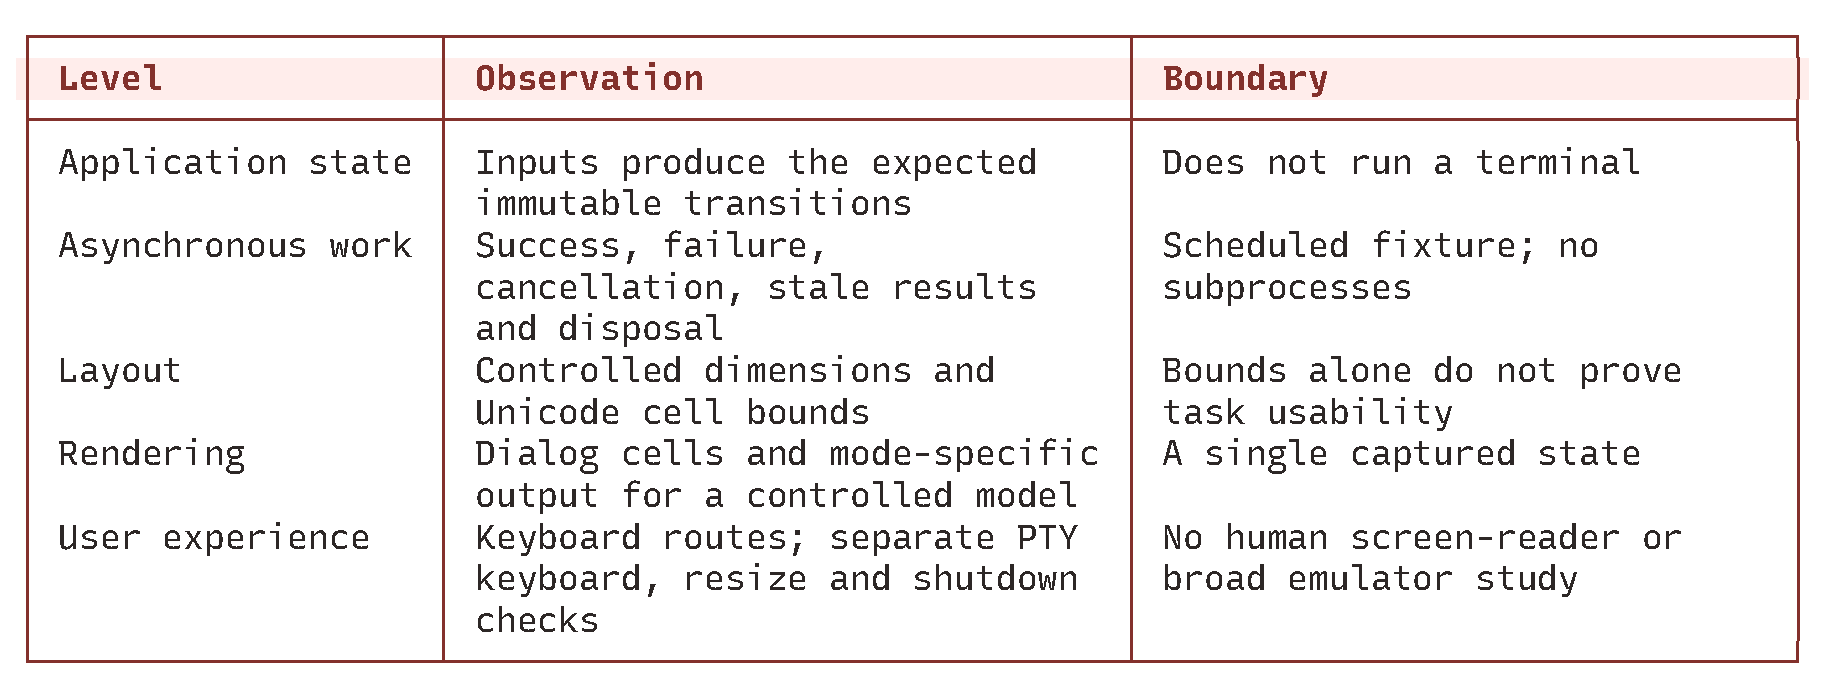
\includegraphics[width=\linewidth]{figures/tables/workshop-evidence-g1-1.pdf}
\par\smallskip{\scriptsize\color{BookMuted}Rows 1–5. Actual Bijou table component.}
\end{center}


\subsection{State and effects}

A state test starts a job, applies progress and checks the result. It also sends a late completion after cancellation and restart. This proves that the transition rejects the old run under those inputs. The scheduler test advances known delays, observes success and failure, cancels work and disposes the driver. It establishes which messages are emitted, including the absence of later messages after disposal.

Those tests do not establish the behavior of an operating-system process runner. The example has none. Replacing the scheduled fixture with subprocesses introduces buffering, exit codes, signal delivery and process-tree ownership that require their own adapter checks.

\subsection{Geometry and cells}

The layout test checks controlled widths and heights, including wide characters, combining text and an emoji sequence. The routing test supplies actual Bijou framework messages to the App and inspects the Surface produced for cancellation. These checks connect input, state and rendering. They still cannot tell whether a human notices the prompt, understands a failure message or can navigate effectively with a particular assistive tool.

\section{Read failure as information}

\subsection{Make the broken state reproducible}

The four exercise fixtures fail intentionally: modal input leaks, a stale result replaces current detail, a colored mark loses meaning, and work emits after closure. Each has a small command, a fixed starting state and an observable success criterion. The repaired path uses the production implementation. Default CI runs the ordinary suite and the repaired exercises; it does not mistake an intentionally broken teaching fixture for a regression in the final application.

\subsection{Avoid convenient evidence substitutions}

A typecheck does not establish a temporal property. A screenshot does not establish input ownership. A cell-bound test does not establish that every control remains reachable. A keyboard-routing test does not establish how a screen reader announces the application. Keep the attractive artifact and the behavioral evidence together while naming what each establishes.

\section{Read the decisions and their costs}

\subsection{Semantic styling}

The problem is a useful state disappearing when color disappears. A tempting shortcut is to make red mean failure by itself. The chosen starting point is textual state with optional visual reinforcement. This spends columns and can feel less compact. It preserves a fact that every mode can carry. Semantic tokens become useful when styling is added: the role remains ``error'' while a theme chooses its appearance.

\subsection{Explicit ownership}

The problem is an action reaching a page behind its dialog or a result reaching a screen that no longer owns it. Global shortcuts and unqualified callbacks look simple until those owners diverge. The chosen model makes input boundaries, run identities and view epochs explicit. The cost is more state and more transitions to test. The benefit is an ownership claim that can be examined before a convincing frame hides the defect.

\subsection{Meaning separate from presentation}

The problem is a consumer needing facts that were stored only as a rendered string. Keeping an immutable model and several formatters adds code paths and compatibility obligations. It also lets the same failed job appear in a table, a CI snapshot, TSV and explicit accessible prose without reconstructing its identity from decoration. Every added presentation must preserve the task's agreed facts; sharing a model does not make a formatter correct automatically.
%
\chapter*{Workshop 7: Ship a reproducible example}\label{workshop-07}
\addcontentsline{toc}{chapter}{W7: Ship a reproducible example}

\section{Pin the thing a reader can actually run}

The companion lives in its own public repository: \url{https://github.com/flyingrobots/bijou-job-monitor}. This edition uses tag \texttt{book-v1} and the exact commit recorded on the version page. The package lock pins published Bijou 7.2.0 and the supporting toolchain. The archived records elsewhere in the book discuss several versions and aspirations; they are not the dependency manifest for this application.

\subsection{Reproduce a checkpoint}

Clone the repository, check out the recorded commit or edition tag, and run \texttt{npm ci}. Run the checkpoint command for the workshop being read, then its checks. The first two checkpoints display a model and its modes. The third opens the complete interactive application. The fourth reproduces stale-result rejection, and the fifth exercises narrow layout and expanded text. The sixth workshop runs the test evidence; this workshop inspects packaging. The checkpoints share the finished modules instead of maintaining five independent copies that can drift.

This is a reproducible route through the construction, not a claim that every checkpoint is a separate historical release. When making an incompatible change to an example, create another edition tag and update the book's recorded reference. A reader should be able to return to the code that produced the explanation.

\subsection{Verify the distributed source}

Run \texttt{npm pack --dry-run} and inspect the listed files. The code package includes the full Apache 2.0 license, its NOTICE, source-file copyright statements, checkpoints and exercises. Git checkout also retains the package lock. Dependencies retain their own applicable notices if they are redistributed with a package. The copyright page in the book does not replace these files.

\section{Keep claims attached to their environment}

\subsection{An environment record has limits}

The version page identifies Node, npm, the companion commit, the published Bijou release and the locally tested host. The companion's \path{VERIFICATION.json} records fifteen passing tests and the pseudo-terminal observations. GitHub Actions runs the pinned checks on Linux; its current result belongs to that run and should be read from the repository. No human screen-reader session or broad terminal-emulator matrix was performed for this edition. Those are open acceptance questions rather than implied guarantees.

\subsection{Make corrections findable}

Use the companion's issue tracker for book-example errata. Include the workshop, edition commit, command, environment, expected result and observed result. A correction becomes more useful when another reader can reproduce it. Keep the original edition available while a later edition explains the repair and its compatibility effect.

\section{Let the book be a working specimen}

The monitor already lets readers start jobs, switch to logs, change selection, filter failures and resize the view. The explicit CLI modes let them inspect the same fixture as static text, TSV or accessible prose. Its tests expose state and cells without requiring an image. The printed explanations remain complete; the running application supplies another way to examine their claims.

A future inspector could make model snapshots and layout rectangles visible inside the application. That capability is not implemented in this checkpoint. It should be added when it answers a concrete learning question and arrives with its own evidence. The useful flourish is the connection between the explanation and a working surface, not an unverified menu promising every debugging feature.
%
